\documentclass[12pt]{article}
\usepackage{fullpage,enumitem,amsmath,amssymb,graphicx}

\begin{document}

\begin{center}
{\Large CS221 Fall 2018 Homework [blackjack]}

\begin{tabular}{rl}
SUNet ID: & prabhjot \\
Name: & Prabhjot Singh Rai \\
Acknowledgement for having formed study group with: & Amey Naik (Project mate)
\end{tabular}
\end{center}

By turning in this assignment, I agree by the Stanford honor code and declare
that all of this is my own work.

\section*{Problem 1}

\begin{enumerate}[label=(\alph*)]
  \item 
  The equation $V_{opt}$  is given by: \\
  \begin{align*}
  V_{opt} = \begin{cases} 
  0 & \text{if $endState$} \\
  max_{\text{a } \epsilon \text{ actions}} Q_{opt}(s, a) & \text{otherwise}
  \end{cases}
  \end{align*}
  where,
  $$Q_{opt}(s, a) = \sum_{s'} T(s, a, s')[\text{Reward}(s, a, s') + \gamma V_{opt}(s')]$$
  \textbf{Iteration 0} \\
  As per the question, $V$ is assigned values of $0$. Therefore,
  $$V_{opt} = \{-2: 0, -1: 0, 0: 0, 1: 0, 2: 0\}$$
 \textbf{Iteration 1}
 \begin{enumerate}
 	\item State $0$ \\
 	\begin{enumerate}
 		\item Action $+1$ \\
 		\begin{align*}
 		Q_{opt} &= 0.3 * [-5 + 0] + 0.7 * [-5 + 0] \\
 		&= -5
 		\end{align*}
 		\item Action $-1$ \\
 		\begin{align*}
 		Q_{opt} &= 0.8 [-5 + 0] + 0.2 * [-5 + 0] \\
 		&= -5
 		\end{align*}
 	\end{enumerate}
 	Therefore, $V_{opt}^1(0) = -5$
 	\item State $1$ \\
 	\begin{enumerate}
 		\item Action $+1$
 		\begin{align*}
 		Q_{opt} &= 0.3 * [100 + 0] + 0.7 * [-5 + 0] \\
 		&= 26.5
 		\end{align*}
 		\item Action $-1$
 		\begin{align*}
 		Q_{opt} &= 0.8 * [-5 + 0] + 0.2 * [100 + 0] \\
 		&= 16
 		\end{align*}
 	\end{enumerate}
 	Therefore, $V_{opt}^1(1) = 26.5$
 	\item State $-1$ \\
 	\begin{enumerate}
 		\item Action $+1$
 		\begin{align*}
 		Q_{opt} &= 0.3 * [-5 + 0] + 0.7 * [20 + 0] \\
 		&= 12.5
 		\end{align*}
 		\item Action $-1$
 		\begin{align*}
 		Q_{opt} &= 0.8 * [20] + 0.2 * [-5] \\
 		&= 15
 		\end{align*}
 		Therefore, $V_{opt}^1(-1) = 15$
 	\end{enumerate}
 	\item State $2$, since it's an end state $V_{opt}^1(2) = 0$
 	\item State $-2$, since it's an end state $V_{opt}^1(-2) = 0$
 \end{enumerate}
 Therefore,
 $$V_{opt}^1 = \{ -2:0, -1: 15, 0: -5, 1: 26.5, 2:0 \}$$
 \textbf{Iteration 2}
 \begin{enumerate}
 \item State $0$
 \begin{enumerate}
	\item Action $+1$
	 \begin{align*}
	 Q_{opt} &= 0.3 * [-5 + 26.5] + 0.7 * [-5 + 15] \\
	 &= 6.45 + 7 \\
	 &= 13.45
	 \end{align*} 
	 \item Action $-1$
	 \begin{align*}
	 Q_{opt} &= 0.8 * [-5 + 15] + 0.2 * [-5 + 26.5] \\
	 &= 8 + 4.3 \\
	 &= 12.3
	 \end{align*}
 \end{enumerate}
 Therefore, $V_{opt}^2(0) = 13.45$
 \item State $1$
	\begin{enumerate}
		\item Action $+1$ \\
			\begin{align*}
				Q_{opt} &= 0.3 * [100 + 0] + 0.7 * [-5 + -5] \\
				&= 30 - 7 \\
				&= 23
			\end{align*}
		\item Action $-1$ \\
			\begin{align*}
				Q_{opt} &= 0.8 * [-5 + -5] + 0.2 * [100 + 0] \\
				&= -8 + 20 \\
				&= 12
			\end{align*}
	\end{enumerate}
	Therefore, $V_{opt}^2(1) = 23$
\item State $-1$
	\begin{enumerate}
		\item Action $+1$
			\begin{align*}
				Q_{opt} &= 0.3 * [-5 + -5] + 0.7 * [20] \\
				&= -3 + 14 \\
				&= 11
			\end{align*}
		\item Action $-1$
			\begin{align*}
				Q_{opt} &= 0.8 * [20] + 0.2 * [-5 + -5] \\
				&= 16 - 2 \\
				&= 14
			\end{align*}
	\end{enumerate}
	Therefore, $V_{opt}^2(-1) = 14$
 \end{enumerate}
 Therefore, $$V_{opt}^2 = \{ -2: 0, -1: 14, 0: 13.45, 1: 23, 2: 0\}$$
  \item From the solution in $1a$, the different [Action, $Q_{opt}(s,a)$] after iteration 2 for
  	\begin{enumerate}
  		\item State $0$ = $[+1, 13.45] [-1, 12.3]$, therefore, $\pi_{opt}(0) = +1$
  		\item State $1$ = $[+1, 23] [-1, 12]$, therefore, $\pi_{opt}(1) = +1$
  		\item State $-1$ = $[+1, 9] [-1, 14]$, therefore, $\pi_{opt}(-1) = -1$
  	\end{enumerate}
  	Therefore, $$\pi_{opt}(s) = \{ -1: -1, 0: +1, 1: +1 \}$$
\end{enumerate}

\section*{Problem 2}

\begin{enumerate}[label=(\alph*)]
	\addtocounter{enumi}{1}
	\item If we have an acyclic MDP, that means there is no way to start at any state $s$ and follow a consistently-directed sequence of edges that eventually loop back to $s$ again. Thus, at any given state, in the calculation of $V_{opt}$, there's no recurrent term. For the end states, we know that $V_{opt}$ is $0$. We can start from states who's chance nodes lead to terminal state, and start calculating $Q_{opt}$ for them(with the help of which we can calculate $V_{opt}$). Next, we calculate $Q_{opt}$ for states whose chance nodes end in state for which we have already calculated $V_{opt}$. Hence, the algorithm calculates $V_{opt}$ for every state in the reverse order in a single pass over all $(s,a,s')$ triples.
	Brief description of the algorithm is as below. Let $D$ be the depth of the tree. $S_{n}^d$, denotes the states at the depth $d$ and value of $V_{opt}$ for all states $S_{n}^D$ is 0.
	\begin{align*}
	\text{while $d$ goes from $D-1$ to $0$:} \\
	\forall S_{n}^d, V_{opt}(S_{n}^d) = max_{\text{a }\epsilon \text{ actions}}(Q_{opt}(S_{n}^d, a)) \\
	\end{align*}	
	where \\
	\begin{align*}
	Q_{opt}(S_{n}^d, a) = \sum T(s^d,a,s^{d+1}) (\textbf{Reward}(s^d,a,s^{d+1}) + \gamma V_{opt}^{d+1})
	\end{align*}
	\begin{center}
	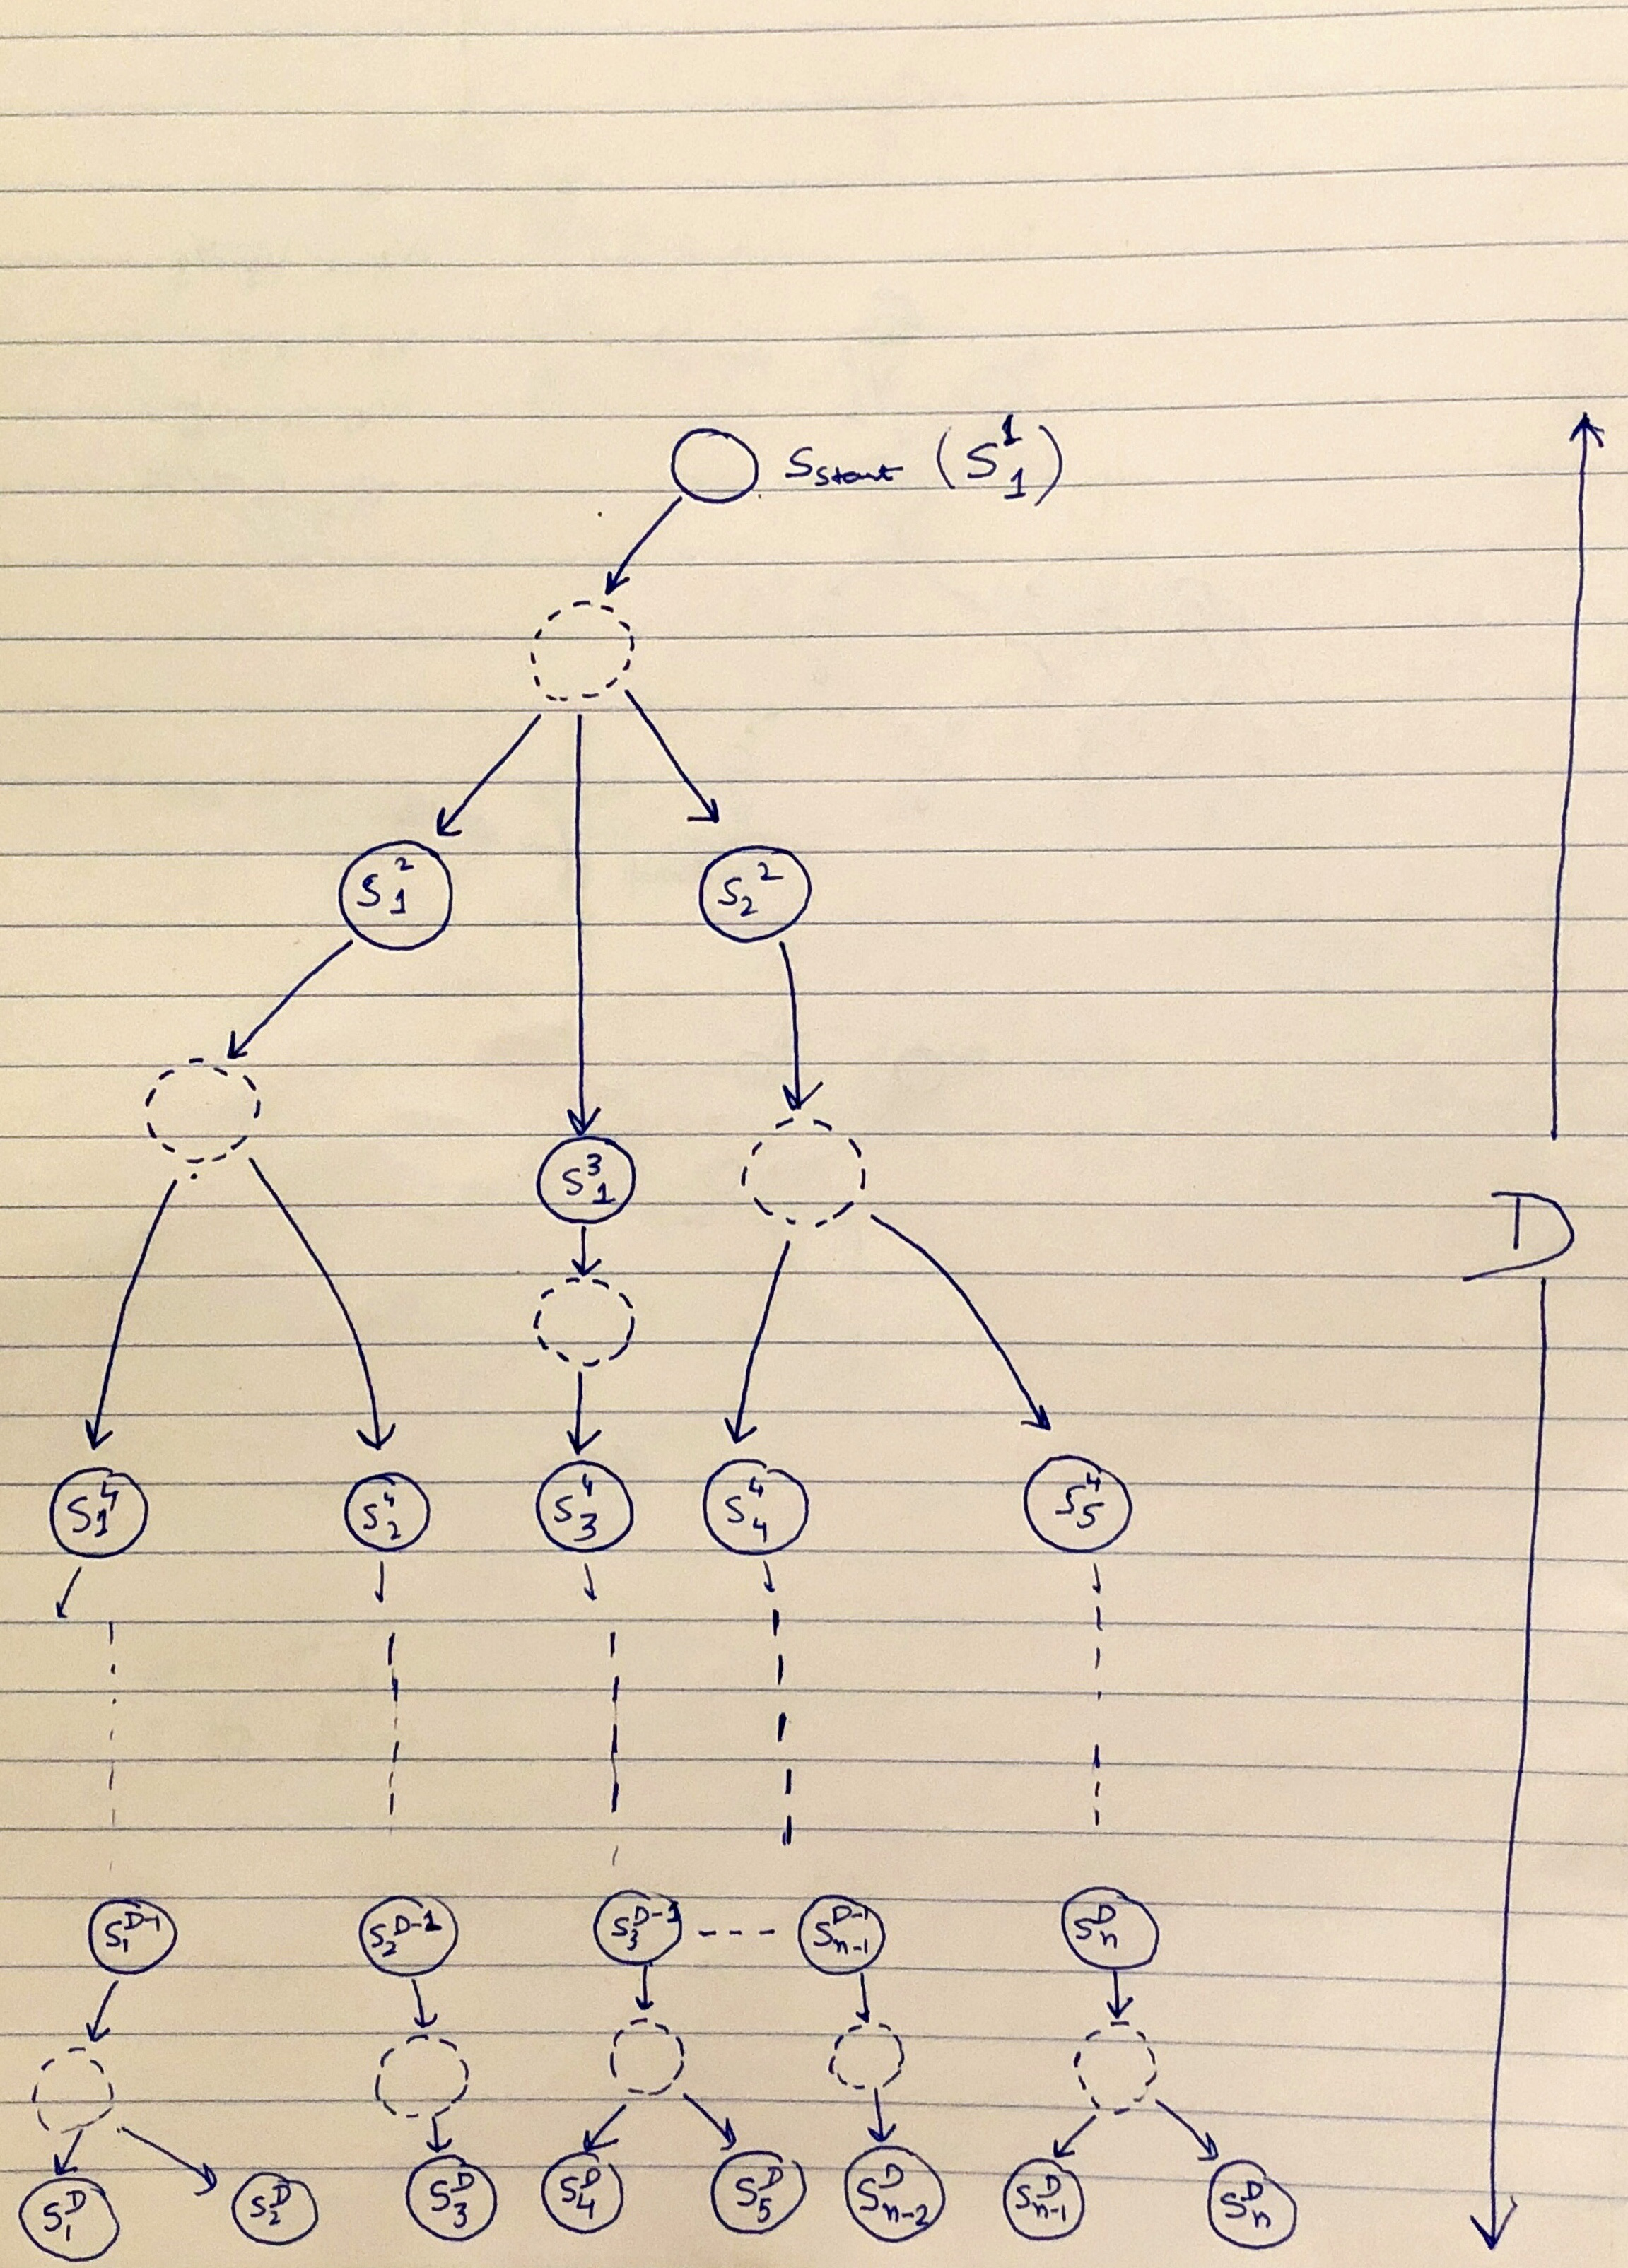
\includegraphics[scale=0.1]{IMG_2203.png}
	\end{center}
	\item The given MDP solver solves the equation when $\gamma = 1$. It means it can solve the equation of the form:
	\begin{align*}
	V_{opt} &= \begin{cases}
	0 & \text{  if $isEnd$} \\
	max_{\text{a } \epsilon \text{ actions}} Q_{opt}(s, a) & \text{  otherwise} \\
	\end{cases} \\
	Q_{opt} (s, a) &= \sum_{s'} T(s, a, s')[\text{Rewards} (s,a,s') + V_{opt}(s')]
	\end{align*}
	The problem statement to solve is: \\
	\begin{align*}
	V'_{opt} &= \begin{cases}
	0 & \text{  if $isEnd$} \\
	max_{\text{a } \epsilon \text{ actions}} Q'_{opt}(s, a) & \text{  otherwise} \\
	\end{cases} \\
	Q'_{opt} (s, a) &= \sum_{s'} T(s, a, s')[\text{Rewards} (s,a,s') + \gamma V'_{opt}(s')] \\
	&=\sum_{s'} \gamma T(s, a, s') [\frac{\text{Rewards} (s,a,s')}{\gamma} + V'_{opt}(s')] & \textbf{(...1)} \\
	\end{align*}
	The above equation looks similar to what the given MDP solver can compute, but since in the above equation, the probabilities do not sum to 1 but to $\gamma$, we need to insert a new state which sums the probabilities to 1. Therefore, we can think of adding extra transition to the list of transitions from a given chance node (or given state) to a new state $o$, such that it conforms to the modified above equation 1 and at the same time, is mathematically correct. As given in the question, we need to make sure that the optimal values $V_{opt}$ for all s $\epsilon$ States are equal under the original and the new MDP. Therefore, $V'_{opt}(s')$ should be equal to zero, which will be possible only when we transition to end state. Moreover, we can set the Reward to transition to this state as 0. Hence,
	\begin{align*}
	Q'_{opt} (s, a) &= \sum_{s'} \gamma T(s, a, s') [\frac{\text{Rewards} (s,a,s')}{\gamma} + V'_{opt}(s')]  + (1-\gamma) [\text{Reward} (s, a, o) + V'_{opt}(o)] \\
	\end{align*}
	where Reward$(s,a,o) = 0$ and $V'_{opt} = 0$(since it's an end state).
	Hence, in order to solve the new MDP with $\gamma$ using the MDP solver for $\gamma = 1$, we need to multiply all the transition probabilities with $\gamma$ and divide the given rewards by $\gamma$. \\
	\begin{align*}
		T'(s,a,s') &= T(s,a,s') * \gamma \\
		\text{Reward'} (s,a,s') &= \frac{\text{Reward} (s,a,s')}{\gamma}
	\end{align*}	 
\end{enumerate}

\section*{Problem 3}

\begin{enumerate}[label=(\alph*)]
	\addtocounter{enumi}{1}
	\item For small MDP and identity feature extractor, we observe high similarity in the Q-learning policy and value iteration policy. The actions are same in around $96\%$ of the cases.  But the accuracy when we use larger MDP and the identity feature extractor drastically decreases to around $68\%$. \\
	The reason for lower performance on larger MDP is that when the number of states are higher and our feature extractor is keeps only (state, action) tuples as features, q-learning for given iterations cannot visit all the possible states in the given iterations and can't learn the right weights. This is the specific problem of generalization. For the small MDP, the total weights are equal to the number of (state, action) pairs(both 81) as the simulation for q learning can visit all the states in the given iterations and update the weights accordingly, hence we get higher accuracy. But for the larger MDP, the total number of (state,action) pairs possible are around 8235, whereas our total weights for the given iteration are around 2000. Therefore, the identity feature extraction based on state and action is not a good solution since it doesn't create generic features which can be applied even if the state is an unseen state, hence poor performance.
	\addtocounter{enumi}{1}
	\item Output from the code by running $4d-helper$:
	
	Expected Reward on modified mdp using original mdp policy: $6$ \\
	Expected Reward on modified mdp using Q Learning: $10$ \\
	
	When we simulate the blackjack game for the modified MDP of higher threshold using the optimum policy learnt through Value Iteration on original MDP of lower threshold, since the algorithm isn't incorporating any feedback(is a fixed algorithm on a given policy), it will play according to the old threshold of 10. And the expected reward will be the same as if it was playing the old game of threshold 10 and not 15 (expected reward being around 6 in both cases). \\ \\
	Once we replace the learning algorithm to RL learning algorithm, it will start incorporating feedback from some random actions and some optimum actions, and use them improve it's feature weights through learning from episodes on the actual threshold directly. Since it will follow exploration and exploitation approach on a threshold of 15, we see higher expected reward of around 10 in this case.
\end{enumerate}

\end{document}